\documentclass{article}

\usepackage{etex}               % must be include as the first package, otherwise an error will appear
\usepackage[margin=1in]{geometry}

\usepackage{float}
\restylefloat{table}

\usepackage{graphicx}
\usepackage{url}
\usepackage{harmony}
\usepackage{musixtex}
\usepackage{subfigure}
\usepackage{caption}
\usepackage[usenames,dvipsnames,svgnames,table]{xcolor}
\usepackage{listings}
\usepackage{alltt}
\usepackage{amsmath}

\usepackage{syntax}
\renewcommand{\syntleft}{\normalfont\itshape}
\renewcommand{\syntright}{}

\usepackage{amssymb}
\usepackage{verbatimbox}

\usepackage{pgf}
\usepackage{tikz}
\usepackage{qtree}
\usepackage{tikz-qtree}
\tikzstyle{vertex}=[draw,fill=black!15,circle,minimum size=20pt,inner sep=0pt]
\usetikzlibrary{arrows, automata, backgrounds, decorations, fit}
\usepackage[latin1]{inputenc}

\tikzset{
    fill background/.style={background rectangle/.style={fill=shadecolor},
        show background rectangle},
         data layout/.style={background rectangle/.style={fill=beige},
             show background rectangle,inner frame xsep=0pt, x=6.5pt,y=12pt},
         solidoutline/.style={very thick, draw, fill=white},
         mux2/.style={shape=trapezium, solidoutline, shape border rotate=180,
             trapezium angle=70, minimum height=8pt},
         op/.style={shape=circle, solidoutline, minimum width=12pt,
             minimum height=12pt, inner sep=0pt},
         ff/.style={shape=rectangle, fill=black, inner sep=0pt, minimum height=2pt, minimum width=8pt},
}

%\usepackage{biblatex}
%\usepackage{subcaption}

\title{\Large SMURF Programming Language Final Report} 

\author{\normalsize Richard Townsend, Lianne Lairmore, Lindsay Neubauer, Van Bui, Kuangya Zhai
	\\ \small \{rt2515, lel2143, lan2135, vb2363, kz2219\}@columbia.edu \vspace{0.6cm}}

\date{\today \vspace{2cm}}

\begin{document}

\definecolor{mygreen}{rgb}{0,0.6,0}
\definecolor{mygray}{rgb}{0.5,0.5,0.5}
\definecolor{mymauve}{rgb}{0.58,0,0.82}

\lstset{ %
	    backgroundcolor=\color{white},   % choose the background color; you must add \usepackage{color} or \usepackage{xcolor}
	    %basicstyle=\footnotesize,       % the size of the fonts that are used for the code
	    basicstyle=\scriptsize\ttfamily, 		     % the size of the fonts that are used for the code
		breakatwhitespace=false,         % sets if automatic breaks should only happen at whitespace
		breaklines=true,                 % sets automatic line breaking
		captionpos=b,                    % sets the caption-position to bottom
		commentstyle=\color{mygreen},    % comment style
		deletekeywords={...},            % if you want to delete keywords from the given language
		escapeinside={\%*}{*)},          % if you want to add LaTeX within your code
		extendedchars=true,              % lets you use non-ASCII characters; for 8-bits encodings only, does not work with UTF-8
		frame=single,                    % adds a frame around the code
		keepspaces=true,                 % keeps spaces in text, useful for keeping indentation of code (possibly needs columns=flexible)
		keywordstyle=\color{blue},       % keyword style
		language={[Objective]Caml},	     % the language of the code
		morekeywords={*,...},            % if you want to add more keywords to the set
		numbers=left,                    % where to put the line-numbers; possible values are (none, left, right)
		numbersep=5pt,                   % how far the line-numbers are from the code
		numberstyle=\tiny\color{mygray}, % the style that is used for the line-numbers
		rulecolor=\color{red},           % if not set, the frame-color may be changed on line-breaks within not-black text (e.g. comments (green here))
		showspaces=false,                % show spaces everywhere adding particular underscores; it overrides 'showstringspaces'
		showstringspaces=false,          % underline spaces within strings only
		showtabs=false,                  % show tabs within strings adding particular underscores
		stepnumber=5,                    % the step between two line-numbers. If it's 1, each line will be numbered
		stringstyle=\color{mymauve},     % string literal style
		tabsize=2,                       % sets default tabsize to 2 spaces
		title=\lstname                   % show the filename of files included with \lstinputlisting; also try caption instead of title
}

\lstdefinestyle{makefile}
{
    numberblanklines=false,
    language=make,
    tabsize=4,
    keywordstyle=\color{red},
    identifierstyle= %plain identifiers for make
}

\maketitle

\section{Introduction}

SMURF is a functional language that allows a composer to create serialist music
based on the twelve tone composition technique. In general, serialism is a musical composition
method where a set of values, chosen through some methodical progress,
generates a sequence of musical elements. SMURF is based on the
functional syntax and semantics set forth by Haskell. The backend of
SMURF generates MIDIs corresponding to the composition defined by the 
user's initial program in SMURF. 


\subsection{Background: What is Serialism?}

In general, serialism is a musical composition technique where a set of values, chosen through some 
methodical process, generates a sequence of musical elements. Its origins are often attributed to
Arnold Schoenberg's twelve-tone technique, which he began to use in the 1920s. In this system, 
each note in the chromatic scale is assigned an integer value, giving us a set of twelve
``pitch classes'' (Figure~\ref{fig:pc}~\cite{appleby2013accidentals}). A composer utilizing this 
method then takes each of these integers, and orders them into a $twelve$ $tone$ $row$, where 
each number appears exactly once. We refer to this row as the $prime$ $form$ of a piece, 
and conventionally refer to it as $P_0$. 

\begin{figure}
\begin{minipage}{0.6\textwidth}
	\centering
	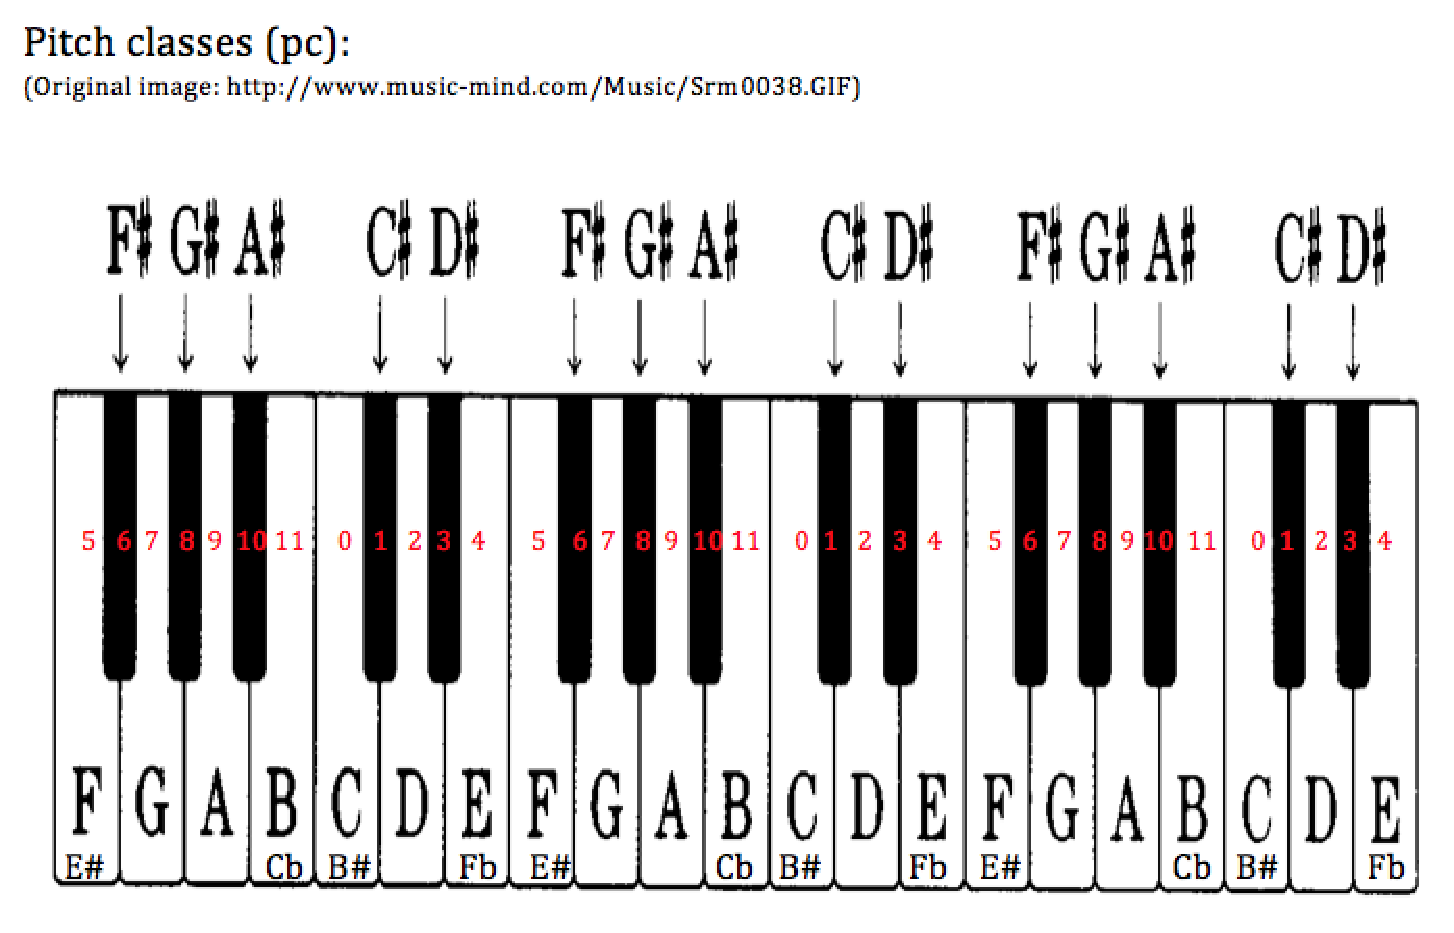
\includegraphics[width=\textwidth]{figures/serialismPianoImage}
	\caption{pitch classes}
	\label{fig:pc}
\end{minipage}\hfill
\begin{minipage}{0.4\textwidth}
	\centering
		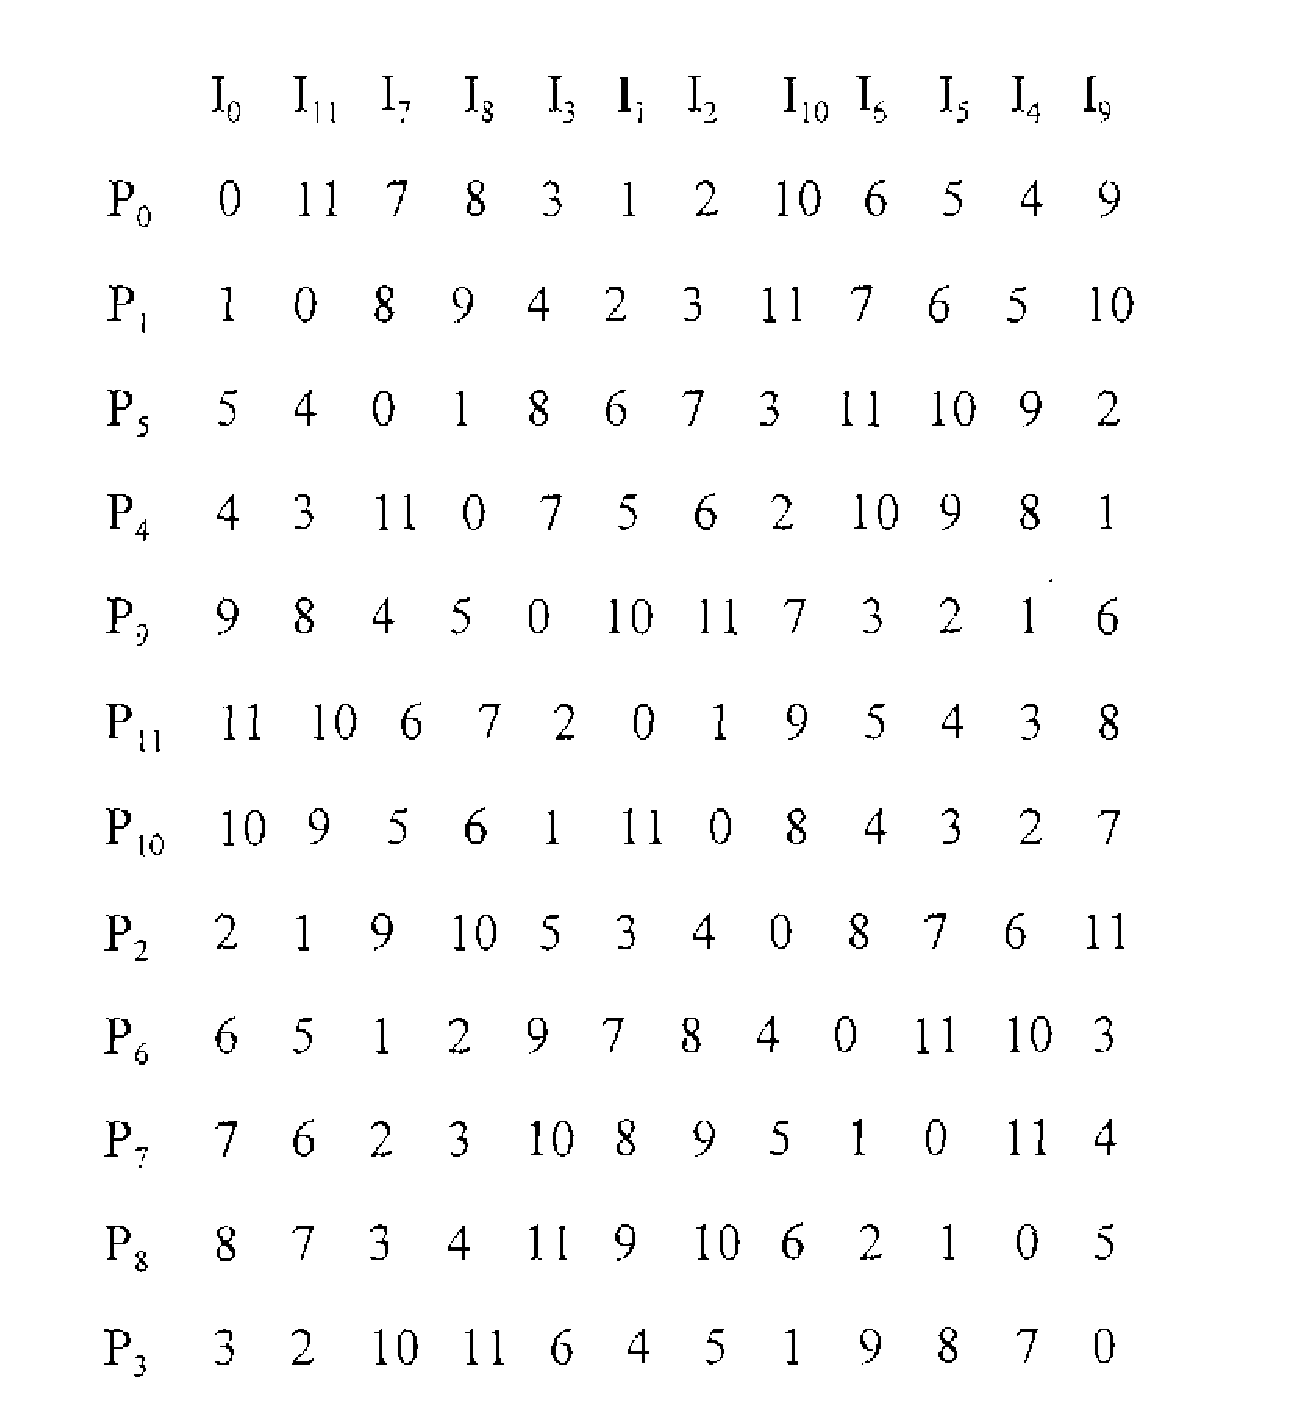
\includegraphics[width=\textwidth]{figures/12_tone}
	\caption{twelve tone matrix}
	\label{fig:12tone}
\end{minipage}
\end{figure}


The composer can then generate other rows that are derived from $P_0$ through three types of transformations:
transposition, inversion, and retrograde. In each of these transformations, we always use mod 12 arithmetic to preserve the 
numbering system of our pitch classes. Transposing a row consists of taking each pitch class in the row and adding the same number 
to each. If we transpose $P_0$ by four semitones, we add four mod twelve to each pitch class in $P_0$ and end up with a new row 
called $P_4$. In general, $P_x$ is a transposition of $P_0$ by $x$ semitones. To invert a row, we "flip" each interval between two 
pitch classes in that row. An interval is best thought of as the smallest "distance" between two pitch classes, using the proximity
on the piano of the two pitch classes as the distance metric (refer to Figure 1 for reference). 
For example, pitch classes 0 and 11 have a distance of 1 from each other,
since you can reach pitch class 0 from 11 by adding 1 to 11 (remember the mod 12 arithmetic) or reach 11 from 0 by subtracting 1
from 0. Thus an interval of +1 exists from 11 to 0, and an interval of -1 exists from 0 to 11.
As a further example, if $P_0$ starts with pitch classes 0-11-7, then we have an interval of -1 between the first two 
pitches and -4  between the second two. Flipping an interval between two pitch classes is identical to
negating its sign.
Thus, in the inverse of $P_0$ (called $I_0$), the first interval would be +1 and the second would 
be +4, giving us 0-1-5 as our first three pitch classes.  The subscript of $I_x$  refers both to the number of transpositions required 
to arrive at $I_x$ from $I_0$, and to the prime row $P_x$ that would need to be inverted to generate $I_x$. The final row 
operation is a retrograde transformation, which merely consists of reading a row backwards. That is, $R_x$ is generated by reading 
the pitch classes of $P_x$ in their opposite order. One can also have a retrograde inversion; $RI_x$ is generated by reading the 
pitch classes of $I_x$ backwards.

Once a composer chooses a $P_0$, the three transformations outlined above can be applied to varying degrees to generate a 
$twelve$ $tone$ $matrix$, which will contain each $P$ row as a row in the matrix and each $I$ row as a column.
Furthermore, all of the $R$ and $RI$ rows are found by reading the rows in the matrix from right to left or the columns 
from bottom to top, respectively. An example of a twelve tone matrix from one of Shoenberg's pieces can be found in 
Figure~\ref{fig:12tone}~\cite{devoto2013twelve}. Finally, using the twelve tone matrix as a guide, the composer picks 
various rows and columns to serve as melodic and harmonic elements in their composition, resulting in a piece of serial music.

\subsection{Motivation}

Twelve tone serialism is a mathematically intensive method of creating music which 
involves mapping notes to numbers. It is natural to work with twelve tone rows 
using a programming language since the method treats notes like numbers that 
can be added and subtracted. SMURF makes twelve tone composition 
easier by using data types and programming paradigms that cater to the needs of a serial composer.
By simplifying the method of inverting, retrograding, and transposing rows, composers can focus 
more on how to exploit new ways to make serial music and worry less about 
creating matrices. 

We chose to implement a functional language because of the clear and 
succinct programs that functional languages produce. In addition, the well known ability
of functional languages to work on lists is advantagous for twelve tone serialism, because
most serial arithmetic operations use rows and columns from the twelve tone matrix as operands. 
As a group we were also interested on how a functional language compiler works. 

Overall we hope to use the simplicity of a functional language to help composers write 
complex, new, and interesting music based on twelve tone serialism. 

\section{Turotial}

\documentclass[dvips, 12pt]{article}

% Any percent sign marks a comment to the end of the line

% Every latex document starts with a documentclass declaration like this
% The option dvips allows for graphics, 12pt is the font size, and article
%   is the style


\usepackage[margin=1in]{geometry}

\usepackage{float}
\restylefloat{table}

\usepackage{graphicx}
\usepackage{url}
\usepackage{harmony}
\usepackage{musixtex}
\usepackage{subfigure}
\usepackage{caption}
%\usepackage{biblatex}
%\usepackage{subcaption}

% These are additional packages for "pdflatex", graphics, and to include
% hyperlinks inside a document.


% These force using more of the margins that is the default style


% Everything after this becomes content
% Replace the text between curly brackets with your own

\title{{\Huge \bfseries SMURF Language Reference Manual} \\ \Large \it Serial MUsic Represented as Functions \vspace{0.6cm}}

\author{\normalsize Richard Townsend, Lianne Lairmore, Lindsay Neubauer, Van Bui, Kuangya Zhai
	\\ \small \{rt2515, lel2143, lan2135, vb2363, kz2219\}@columbia.edu \vspace{0.6cm}}

\date{\today \vspace{2cm}}

% You can leave out "date" and it will be added automatically for today
% You can change the "\today" date to any text you like

\begin{document}
\maketitle
\clearpage


% This command causes the title to be created in the document
\tableofcontents

\section{Syntax Notation}
The syntax notation used in this manual are as follows. Syntactic 
categories are indicated by \emph{italic} type. Literal words and 
characters will be displayed in \texttt{typeset}. Alternatives are listed 
on separate lines. Optional terminal and non-terminals are indicated by the
subscript_{opt}. 


\section{Lexical Conventions}
SMURF programs are lexically composed of three elements: comments, tokens, and whitespace.

\subsection{Comments}
SMURF allows nested, multiline comments in addition to single line comments.
\begin{table} [H]
\centering
\begin{tabularx}{\textwidth}{lXl}
\hline\hline
Comment Symbols & Description & Example \\
\hline\hline
  \texttt{/* */} & Multiline comments, nesting allowed & \texttt{/* This /* is all */ commented */} \\ \hline
  \texttt{//} & Single-line comment & \texttt{// This is a comment} \\ \hline
\end{tabularx}
\end{table}


\subsection{Tokens}
In SMURF, a token is a string of one or more characters that is significant as a group.
SMURF has 6 kinds of tokens: {\it identifiers}, {\it keywords}, {\it constants},
      {\it operators},
{\it separators} and {\it newlines}.

\subsubsection{Identifiers}
\label{sec:identifiers}
An identifier consists of a letter followed by other letters, 
digits and underscores. The letters are the ASCII characters \texttt{a}-\texttt{z} and
\texttt{A}-\texttt{Z}. Digits are ASCII characters \texttt{0}-\texttt{9}. SMURF is case sensitive.

\begin{grammar}
<letter> $\rightarrow$ [`a'-`z' `A'-`Z'] 

<digit> $\rightarrow$ [`0'-`9'] 

<underscore> $\rightarrow$ {`_'} 

<identifier> $\rightarrow$ <letter> (<letter> | <digit> | <underscore>)*
\end{grammar}

\subsubsection{Keywords}
\label{sec:keywords}
Keywords in SMURF are identifiers reserved by the language. Thus, they are not available for
re-definition or overloading by users. 

\begin{table} [H]
	\centering
    \begin{tabular}{ll}
    \hline\hline
    Keywords & Descriptions \\ 
    \hline\hline
      \texttt{Bool} & Boolean data type \\ \hline
      \texttt{Int} & Integer data type \\ \hline
      \texttt{Note} & Atomic musical data type \\ \hline
      \texttt{Beat} & Note duration data type\\ \hline
      \texttt{Chord} & Data type equivalent to \texttt{[Note]} type \\ \hline
      \texttt{System} & Data type equivalent to \texttt{[Chord]} type \\ \hline
      \texttt{True, False} & Boolean constants \\ \hline
      \texttt{let, in} & Allow local bindings in expressions  \\ \hline
      \texttt{if, then, else} & Specify conditional expression, else compulsory  \\ \hline
      \texttt{random} & Generate random numbers \\ \hline
      \texttt{print} & Print information to standard output \\ \hline
      \texttt{main} & Specify the value of a SMURF program\\ \hline
    \end{tabular}
\end{table}


\subsubsection{Constants}
\label{sec:constants}
In SMURF, constants are expressions with a fixed value. Integer literals and
Boolean keywords are the constants of SMURF. 

\setlength{\grammarindent}{6em}
\begin{grammar}
<digit> $\rightarrow$ [`0'-`9'] 

<constant> $\rightarrow$ \texttt{-}? [`1'-`9'] <digit>* \\
												 \texttt{0} <digit>* \\
												\texttt{True} \\
												\texttt{False}
\end{grammar}

\subsubsection{Operators}
SMURF permits arithmetic, comparison, boolean, list, declaration, and row operations, all of which
are carried out through the use of specific operators. The syntax and semantics of all of these
operators are described in sections \ref{sec:postfixop}, \ref{sec:prefixop}, and \ref{sec:binaryop},
except for declaration operators, which are described in section \ref{sec:declarations}.


\subsubsection{Newlines}
SMURF uses newlines to signify the end of a declaration, except
when preceded by the \texttt{\textbackslash} token. In the latter case, the newline is ignored by the compiler 
(see example below). If no such token precedes a newline, then the compiler will treat the newline as
a token being used to terminate a declaration.

\subsubsection{Separators}

\begin{grammar}
<separator> $\rightarrow$ \texttt{,} \\
												  \texttt{\&} \\
													\texttt{\textbackslash}
\end{grammar}

Separators in SMURF are special tokens used to separate other tokens. 
Commas are used to separate elements in a list.
The \texttt{\&} symbol can be used in place of a newline. That is, the compiler
will replace all \texttt{\&} characters with newlines. The
\texttt{\textbackslash} token, when followed by a newline token,
may be used to splice two lines. E.g.
\begin{lstlisting}
genAltChords (x:y:ys) = [(x,Time 4,1)]   \
                        :[(y,Time 4,-1)]:genAltChords ys
\end{lstlisting}
is the same as 
\begin{lstlisting}
genAltChords (x:y:ys) = [(x,Time 4,1)]:[(y,Time 4,-1)]:genAltChords ys
\end{lstlisting}


\subsection{Whitespace}
\label{sec:whitespaces}
{\it Whitespace} consists of any sequence of {\it blank} and {\it tab} characters.
Whitespace is used to
separate tokens and format programs. All whitespace is ignored by the
SMURF compiler. As a result, indentations are not significant in SMURF.


\clearpage

% citations begin here
\bibliographystyle{ieeetr}
\bibliography{ref/refs}


\end{document}

\section{Project Plan}

	\subsection{Processes}
		
		\subsubsection{Planning}
		We had a 2 hour meeting every Wednesday that everyone attended. In these meetings, organized by Richard (our benevolent dictator), we discussed project milestones, delegated responsibilities to each member of the group, designed and updated our design of SMURF, and eventually coded in meetings to allow for discussion of tricky parts of our implementation. We chose milestones based on a review of previous semesters team projects that were successful. 
				
		\subsubsection{Specification}
		Both our Proposal and LRM were completely outlined in our group meetings. Lindsay took notes for the group and pushed them to GitHub so all members had access.  We divided the outlines into equal sections to divide the writing and proof-reading responsibilities: Each group member had a portion to write and a different portion to proofread. Once we started coding, any updates that needed to be made were done by the person coding that portion of the language (regardless of who originally wrote that section of the LRM). 
		
		\subsubsection{Development}
		Each member of our group was given a slice of our language to implement from start to finish. By doing this, we minimized the issues that arise from having to wait for another group member's section of the code to be implemented before being able to start your own. We each followed a similar development process, implementing in the same order the scanner (first), parser, abstract syntax tree, semantic abstract syntax tree, and code generation (last). We used GitHub to track our code but did not utilize its branching features for coding. This was a decision we made to force our code to always be in a compilable/runnable form and to avoid large merging issues at the end of development. Because we divided the language into pieces and had complete ownership of our slice, using the LRM (which we worked on together) as the ultimate reference on how to implement our section was crucial. In the few cases where the LRM specification was unable to be implemented in the way we planned, the owner of that section chose how to most appropriately implement it and then updated the LRM and the rest of the group with the changes.
		
		\subsubsection{Testing}
		At the end of each stage of development, every group member wrote unit tests to ensure their slice of the code worked as anticipated. Our integration testing took the form of several "Hello World" style programs. Any failed tests were addressed as soon as the failure was discovered.
		
	\subsection{Style Guide}
	We conformed to the following coding conventions:
		\begin{itemize}
		\item Indentation: 4 spaces, with multiple indents to differentiate between nested blocks of code 
		\item Maximum Characters per Line: 100 (including indentation)
		\end{itemize}
	
	\subsection{Project Timeline}
	Our project timeline includes \emph{class deadlines} and self imposed deadlines.
		\begin{table}[htdp]
		\begin{tabular}{|l|l|}
		\hline
		Date & Milestone \\ \hline
		09-25-13 & \emph{Proposal due} \\
		10-07-13 & Initial LRM section written \\
		10-09-13 & Initial LRM section proofread \\
		10-27-13 & Full proofread of LRM  completed \\
		10-28-13 & \emph{LRM due} \\
		10-28-13 & Scanner and Parser completed  \\
		11-06-13 & Scanner and Parser tests completed \\
		11-20-13 & Semantic Analyzer completed \\
		11-27-13 & Semantic Analyzer tests completed \\
		12-04-13 & End-to-end "Hello World" compilation succeeds \\
		12-20-13& \emph{Final report due} \\ 
		\hline
		\end{tabular}
		\end{table}
		
	\subsection{Roles and Responsibilities}
		\begin{table}[htdp]
		\begin{tabular}{|l|l|}
		\hline
		Team Member & Responsibilities \\ 
		\hline
		Van Bui & Proposal: Examples \\
					& LRM: Write Parenthetical Expressions, Let Expressions, Type Signatures, \\
					& Pattern Matching \\
					& LRM: Proofread  Description of Precedence, Syntax Notation, Library Functions, \\ 
					& Declarations and Bindings \\
					& Code: Function Application \\
		Lianne Lairmore & Proposal: Motivation \\
									& LRM: Write Description of Precedence, Syntax Notation, Library Functions, \\
									& Declarations and Bindings \\
									& LRM: Proofread Lexical Conventions, Primary Expressions, Meaning of Identifiers \\
									& Code: Literals, Main/Print/Random, Symbol Table/Environment, Polymorphism \\
		Lindsay Neubauer & Note Taker \\
										& Proposal: Language Description\\
										& LRM: Write Curried Applications, Operator Application, Conditionals, Lists, \\
										& Tuples \\
										& LRM: Proofread Parenthetical Expressions, Let Expressions, Type Signatures, \\ 
										& Pattern Matching \\
										& Code: Non-music operators, Notes, Beats, Music operators \\
		Richard Townsend & Group Leader \\
										& Proposal: Background \\
										& LRM:  Write Declarations and Bindings \\
										& LRM: Proofread Curried Applications, Operator Application, Conditionals, Lists, \\
										& Tuples \\
										& Code: Pattern Matching, Bindings, Function Application \\
		Kuangya Zhai & GitHub and LaTeX Go-To Person \\ 
								& Proposal: Generate Latex \\
								& LRM: Write Lexical Conventions, Primary Expressions, Meaning of Identifiers \\
								& LRM:  Proofread Declarations and Bindings \\
								& Code: MIDI generation, List operators, Conditionals, Function Application \\
		\hline
		\end{tabular}
		\end{table} 
		
	\subsection{Software Development Environment}
		We used the following tools and languages:
		\begin{itemize}
		\item Compiler Implementation: OCaml, version 4.01.0
		\item Musical Interface: MIDI
		\item Testing Environment: Shell Scripts
		\item Version Control System: GitHub
		\end{itemize}
	
	\subsection{Project Log}
		\begin{table}[htdp]
		\begin{tabular}{|l|l|}
		\hline
		Date & Milestone \\ 
		\hline
		09-18-13 & Proposal writing sections assigned \\
						& GitHub repository setup \\
		09-25-13 & LRM timeline established \\
		10-02-13 & LRM writing and proofreading sections assigned \\
		10-11-13 & Switch from OpenGL musical score to MIDI music \\
		10-16-13 & Decided on top-level description of SMURF program \\
						& Outlined all acceptable inputs and outputs to a SMURF program \\
						& Assigned vertical slices to team members \\
		10-23-13 & Divided backend into semantic analyzer and translator modules  instead of single "compiler" \\
						& module \\
		11-06-13 & Decided to add polymorphism back into language \\
	   					& Discussed structure of Semantic Analyzer modules \\
		11-08-13 & Semantic analyzer started \\
		11-13-13 & Parser completed \\ 
		11-20-13 & Interpreter Started, changed output of semantic analyzer from sast to beefed up symbol table \\
		11-27-13 & Hello World end-to-end compilation succeeds \\
		12-04-13 & Semantic Analyzer with tests completed \\
		12-20-13 & Interpreters with all tests passing completed \\
		 				& Interesting SMURF program end-to-end compilation succeeds \\
		\hline
		\end{tabular}
		\end{table}
	

\section{Architectural Design}

\subsection{Overview}
The SMURF compiler transforms a SMURF program into a playable MIDI file.
 The compiler first scans the source file, parses 
the resulting tokens, creates an abstract syntax tree, semantically 
checks the abstract syntax tree, translates the tree into 
intermediate code and finally translates this intermediate 
representation into a MIDI file which can be played in most 
media players. 


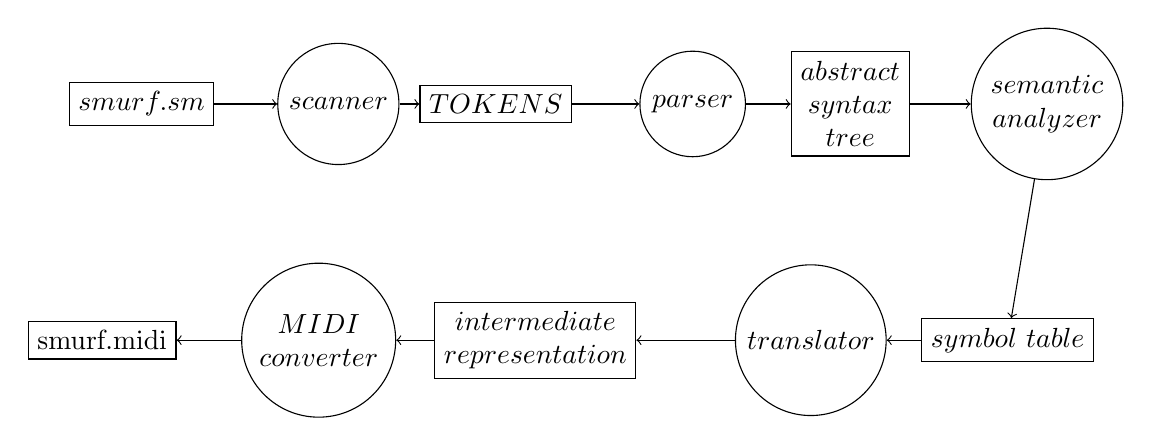
\begin{tikzpicture}[every text node part/.style={align=center}]
\node [draw,shape=rectangle] (smurf) at (0,0) {$smurf.sm$};
\node [draw,shape=circle] (scanner) at (2.5,0) {$scanner$};
\node [draw,shape=rectangle] (tokens) at (4.5,0) {$TOKENS$};
\node [draw,shape=circle] (parser) at (7,0) {$parser$};
\node [draw,shape=rectangle] (ast) at (9,0) {$abstract$ \\ $syntax$ \\ $tree$};
\node [draw,shape=circle] (semanal) at (11.5,0) {$semantic$ \\ $analyzer$};
\node [draw,shape=rectangle] (symtab) at (11,-3) {$symbol$ $table$};
\node [draw,shape=circle] (trans) at (8.5,-3) {$translator$};
\node [draw,shape=rectangle] (ir) at (5,-3) {$intermediate$ \\ $representation$};
\node [draw,shape=circle] (midic) at (2.25,-3) {$MIDI$ \\ $converter$};
\node [draw,shape=rectangle] (midi) at (-.5,-3) {smurf.midi};
\draw [->] (smurf) -- (scanner);
\draw [->] (scanner) -- (tokens);
\draw [->] (tokens) -- (parser);
\draw [->] (parser) -- (ast);
\draw [->] (ast) -- (semanal);
\draw [->] (semanal) -- (symtab);
\draw [->] (symtab) -- (trans);
\draw [->] (trans) -- (ir);
\draw [->] (ir) -- (midic);
\draw [->] (midic) -- (midi);
\end{tikzpicture}

\subsection{Scanner}
The SMURF program file is first passed to the scanner. The scanner 
matches the string of input characters to tokens and white spaces.
The tokens include keywords, constants, and operators used in a SMURF 
program. All white space characters except new lines are ignored. 
Any illegal characters are caught 
and an exception is raised. The tokens are defined with regular 
expressions and nested comments use a state machine and counter 
to be resolved. The scanner was built with the ocaml lexer. 

\subsection{Parser}
The tokens generated in the scanner are then used in the parser. 
The parser matches the string of tokens to a grammar defining the 
SMURF language. An abstract syntax tree is built as the tokens 
are matched to the grammar and stored as a program which is 
defined as a list of declarations. Syntax errors in the 
SMURF code will be identified during parsing resulting 
in an exception being raised. The parser is generated using 
the grammar and the ocaml yacc program. 

\subsection{Abstract Syntax Tree}
The abstract syntax tree is the intermediate representation 
of a SMURF program after it has been parsed but before it has 
been semantically checked. The program can easily be transversed 
by organizing the code into an abstract syntax tree because of its 
hierarchical nature. 

\subsection{Semantic Analyzer}
The semantic analyzer uses the abstract syntax tree to build a 
semantic abstract syntax tree which holds more information like 
scope and type information. Semantic errors are caught during the 
translation and transversing of the semantic abstract syntax tree. 
The semantic analyzer walked through the semantic abstract syntax tree
twice, first to create the symbol table and then to do checks using 
the filled symbol table. The second pass of the semantic abstract 
syntax tree was required because SMURF does not require variables or 
functions to be defined before they are used.  

\subsection{Translator}
The symbol table is then passed to our translator 
which evaluates all expressions and creates an intermediate 
representation that is then converted into MIDI code. 
Since symbol table contains the expression of all 
variables and functions all expressions can be evaluated 
starting from the main declaration without the semantic 
abstract symbol tree. Errors found during evaluation 
of expressions are found causing compilations errors. 
If there are no errors found then an intermediate 
representation is produced. 

\subsection{MIDI Converter}
The intermediate representation produced from the translator then 
is translated into MIDI code using the MIDI converter. The MIDI 
code can then be played. 

\section{Test Plan}

During the development process of SMURF, to let everyone envolve in the development as much as possible, we adopt the slicing model, 
i.e., in each developing stage, everyone has a slice of work to work on.
One problem with this model is that different people need to work on a same job, 
one's change to the program can easily crash other people's work. 
As a result, extensive tests to ensure the quality of the software is crucial. 


The hierachy for SMURF test cases is shown in (figure~\ref{fig:testDir}). 
In each developing stage, everyone is in charge of a directory holding test cases constructed for the functionality he/she is working on. 
Every person needs to give the expect output for his/her test cases in the {\bf exp} directory.
We have a script for testing all the test cases in the toplevel of the direcotry running all the test cases and comparing the results with the expect results given by every owner of the cases. 
The script gives the result about how many test cases passed and which test cases failed, if any. 
Before committing his/her result to the repository, everyone need to make sure the new change passed all the other people's cases. 
For the occasions that one's work need to change the output of other people's cases, 
he/she need to check the changes are as expected, 
and then generate new expected results for the cases before committing changes to repository.


\begin{figure} [H]
\centering
\begin{tikzpicture}[%
grow via three points={one child at (0.5,-0.7) and
    two children at (0.5,-0.7) and (0.5,-1.4)},
    edge from parent path={(\tikzparentnode.south) |- (\tikzchildnode.west)}]

    \node {TEST_ROOT}
    child { node {parser-tests}}     
    child { node {semantic-tests}}
    child { node [selected] {codegen-tests}
        child { node [selected] {person1}
            child{ node {exp}
                child{ node {case1.out} }
                child{ node {case2.out} }
                child{ node {case3.out} }
                child{ node [optional] {...} }
            }
            child [missing] {}              
            child [missing] {}              
            child [missing] {}              
            child [missing] {}              
            child{ node {case1.sm} }
            child{ node {case2.sm} }
            child{ node {case3.sm} }
            child{ node [optional] {...} }
        }
        child [missing] {}              
        child [missing] {}              
        child [missing] {}              
        child [missing] {}              
        child [missing] {}              
        child [missing] {}              
        child [missing] {}              
        child [missing] {}              
        child [missing] {}              
        child { node {person2}}
        child { node {person3}}
        child { node {person4}}
        child { node {person5}}
    };
\end{tikzpicture}
\caption{The direcotry of SMURF test cases}
\label{fig:testDir}
\end{figure}

\subsection{Testing Levels}

\subsection{Test Automation}

\subsection{Example Test Cases}
Below we give several sample test cases and their expected output for SMURF.
\subsubsection{parser-tests}
\lstset{ language=[Objective]Caml }
\lstinputlisting{../../Code/tests/parser-tests/kyzhai/test1.sm}

\subsubsection{semantic-tests}
\lstset{ language=[Objective]Caml }
\lstinputlisting{../../Code/tests/parser-tests/kyzhai/test1.sm}

\subsubsection{codegen-tests}
\lstset{ language=[Objective]Caml }
\lstinputlisting{../../Code/tests/parser-tests/kyzhai/test1.sm}

\section{Lessons Learned}

\subsection{Lindsay Neubauer}
We had a meeting at the same time every week that lasted between one and two hours that everyone attended. This time set aside to make real progress on project was crucial to our success. In the beginning of the semester we spent all the time discussing LRM-related topics and during the latter half of the semester it was split between discussion and coding. Often being in the same room, even for a short amount of time, while coding was helpful for figuring out the trickier aspects of our language. This was particularly helpful for me because OCaml was my first experience using a functional programming language and having access to others with more experience helped me pick it up quicker.
\\ \\
Another important choice we made was to designate a group leader at the beginning of this project. Our group leader was organized with tasks to discuss or complete in each meeting and helped drive the conversation in a productive way. In addition to this, we had a note taker and a person in charge of our GitHub and Latex environments. It was helpful to have �go to� people for questions and concerns that arose throughout the project.
\\ \\
After turning in our LRM we decided to divide each part of our language into slices. Each group member was in charge of a different aspect of our language and implemented that slice for each step of the compiler building process. This ownership of a part of the language was helpful and touching each step of the compiler was very helpful for learning. It also allowed each group member to work throughout the semester regardless of the progress made by others.
\\ \\
The most important learning I had from this project are understanding the functional language paradigm and knowledge on how to implement a compiler from start to finish.

\subsection{Kuangya Zhai}
First of all, the best lesson I learnt from this project is: Finish early. The importance of starting early has been told by numerous previous PLT groups while the importance of finishing early has not. By finishing early I mean you should project the finishing time of the deadline of your project a bit earlier than the actual deadline to allow any exceptions. As is always said, deadline is the first productivity. Your efficiency boosts when the deadline approaching. But there exists the possibility that something unexpected happens and you are not going to be able to finished the project in the due day if your plan is to finish everything in the last day. These situation is common when you are working on a group project. Take our group as an example, we projected everything to be finished on the exact morning of the presentation while it turned out that not everything goes well as expected, so we had to presented an incomplete version which was kind of embarrassing. And the problems was solved on the exact afternoon of the presentation but we had no chance the present it again. Had we project our own deadline one day earlier, I believe the result will be much better. 

The second thing, enjoy OCaml. Few people has functional programming background before the PLT class. So it's likely that you will have a steeper learning curve when comparing with learning other programming languages. However, when you got used to the functional style, you will find it's at least as expressive and productive as imperative languages you have got used to. The thing I love the most about functional programming is its type checking system. So you will spend tons of time to get your program to compile. But once after that, your program will likely to give the correct result since most of the bugs have been captured at the compiling stage. Also, the side effect free property of functional program guarantees the robustness of your program, which is especially important when you are working on a teaming working project. OCaml is not purely functional. It also keeps several imperative features which might also be helpful and make your life much easier when comparing with Haskell, the pure functional programming language. 

\section{Appendix}

\clearpage

\bibliographystyle{ieeetr}
\bibliography{ref/refs}


\end{document}
